\noindent
\begin{tabular}{cc}
\begin{minipage}[b]{0.60\textwidth}
\begin{exerciseS}[Attrazione di due superfici]
Due lamine piane uguali parallele sono separate da una distanza $d$. Tra le lamine è 
presente un sottile strato di liquido. Sono note l'area della superficie $A$ e il perimetro $L$ delle due lamine,
la pressione ambiente $p_a$, la tensione superficiale del liquido $\gamma$ e l'angolo di contatto $\theta$.
Si chiede di determinare la componente perpendicolare alle lamine della forza agente su ciascuna delle due lamine.
\end{exerciseS}
\end{minipage}
&
\begin{minipage}{0.35\textwidth}
   \begin{center}
   \includegraphics[width=0.85\textwidth]{./fig/Plates4}
   \end{center}
\end{minipage}
\end{tabular}

\sol

\partone
 Tensione superficiale. Angolo di contatto.

\parttwo
 La condizione descritta nell'esercizio è una condizione equilibrio. La forza agente su una lamina
è dovuta a due fenomeni: la tensione superficiale sul perimetro del fluido e la differenza di pressione tra fluido 
e ambiente. Si consideri positiva la forza se è una forza di attrazione.

\begin{equation}
  F = F_\gamma + F_p
\end{equation}

\begin{itemize}
  \item Calcolo di $F_\gamma$.
    \begin{equation}
     F_\gamma = \gamma L \sin\gamma
    \end{equation}
  
  \item Calcolo di $F_p$. Il salto di pressione viene calcolato scrivendo l'equilibrio all'interfaccia.
    \begin{equation}
     F_p = (p_a - p) A
    \end{equation}
    con:
    \begin{equation}
     (p_a - p) d = 2 \gamma \cos \theta
    \end{equation}
   
    
  \item La componente totale richiesta risulta quindi:
  \begin{equation}
    F = \frac{2 \gamma A \cos \theta}{d} + L \gamma \sin \theta
  \end{equation}
  
  \begin{center}
     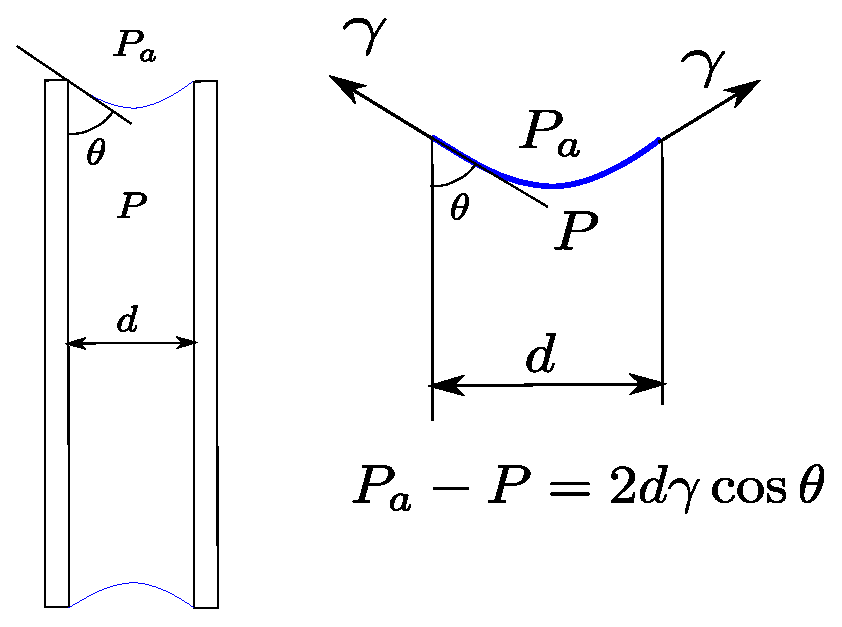
\includegraphics[width=0.50\textwidth]{./fig/sup01.eps}
   \end{center}
     
\end{itemize}
